\chapter{Analisi della PTN}
\label{cap3}
Ora che i dataset sono stati convertiti in una rappresentazione a \textit{grafo} e quindi la rete PTN è un grafo è possibile procedere alla sua analisi.

\section{Analisi spaziale del grafo}
Il grafo potrebbe essere semplicemente visualizzato con una delle topologie classiche dei grafi, ma perderebbe, almeno graficamente, la sua struttura \textit{topologica} reale. È utile infatti non solo visualizzare il grafo, ma anche visualizzarlo con le stesse distanze e la stessa distribuzione che i nodi hanno nella realtà da un punto di vista \textbf{geografico} \cite{Candelieri2019}.

\vspace{1em}
\begin{figure}[h!]
    \centering
    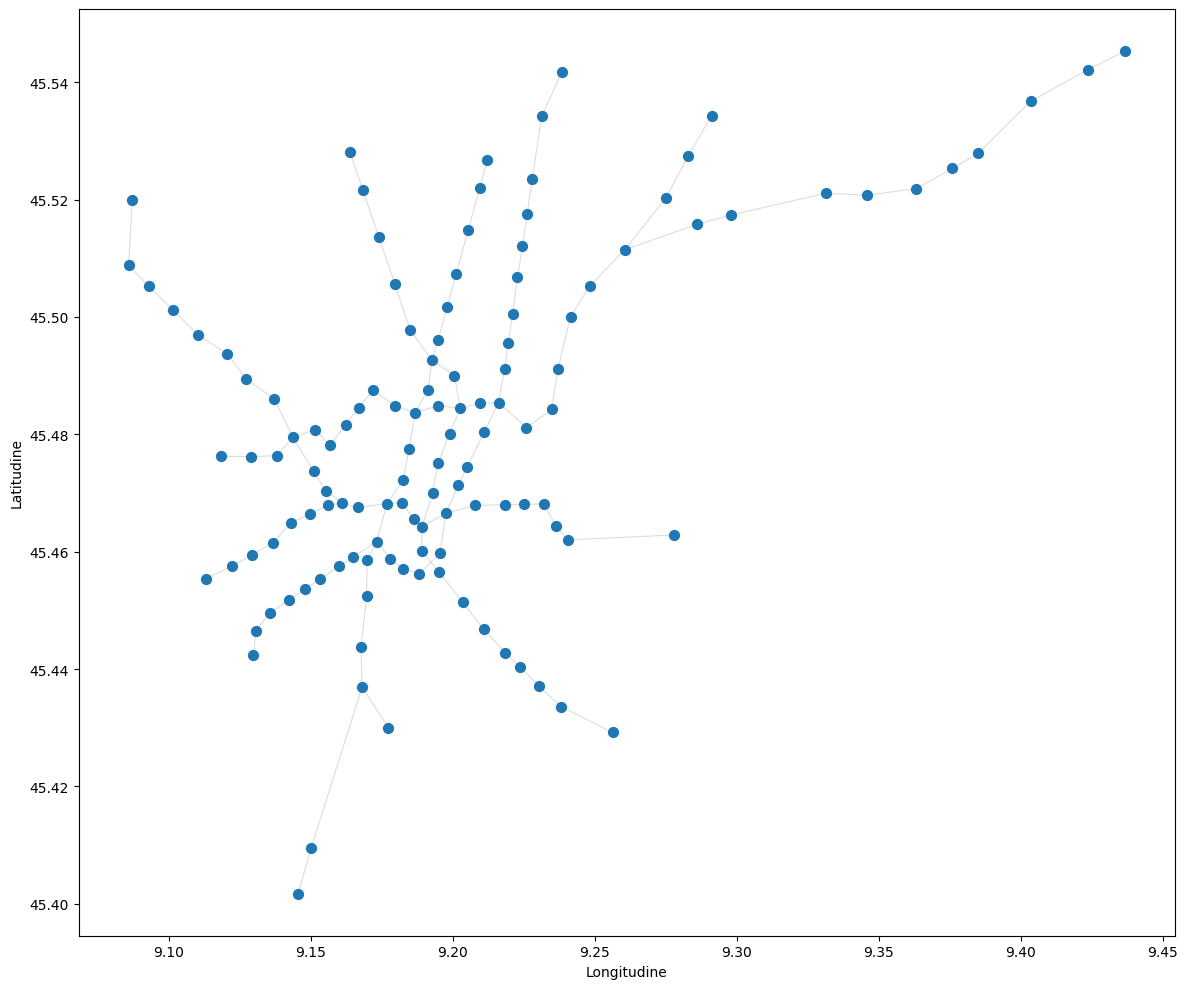
\includegraphics[width=0.8\linewidth]{Immagini//Capitoli//cap3/rete_atm.png}
    \caption{Rete Metropolitana di Milano}
    \label{fig:Rete Metropolitana di Milano}
\end{figure}
\vspace{1em}

Per questa ragione si sono utilizzate le informazioni disponibili di \textbf{latitudine} e \textbf{longitudine} per ottenere la rappresentazione del grafo completo in figura \ref{fig:Rete Metropolitana di Milano}.

\subsection{Analisi spaziale dei sottografi}
Oltre al grafo principale, è possibile visualizzare anche dei \textit{sottografi} corrispondenti alle singole linee metropolitane, discriminando nodi e archi sulla base dell'attributo \texttt{lines} che identifica, appunto, a quale delle linee appartengono.

\vspace{1em}
\begin{figure}[htbp]
  \centering
  % --- Riga 1 ---
  \begin{subfigure}[b]{0.40\textwidth}
    \centering
    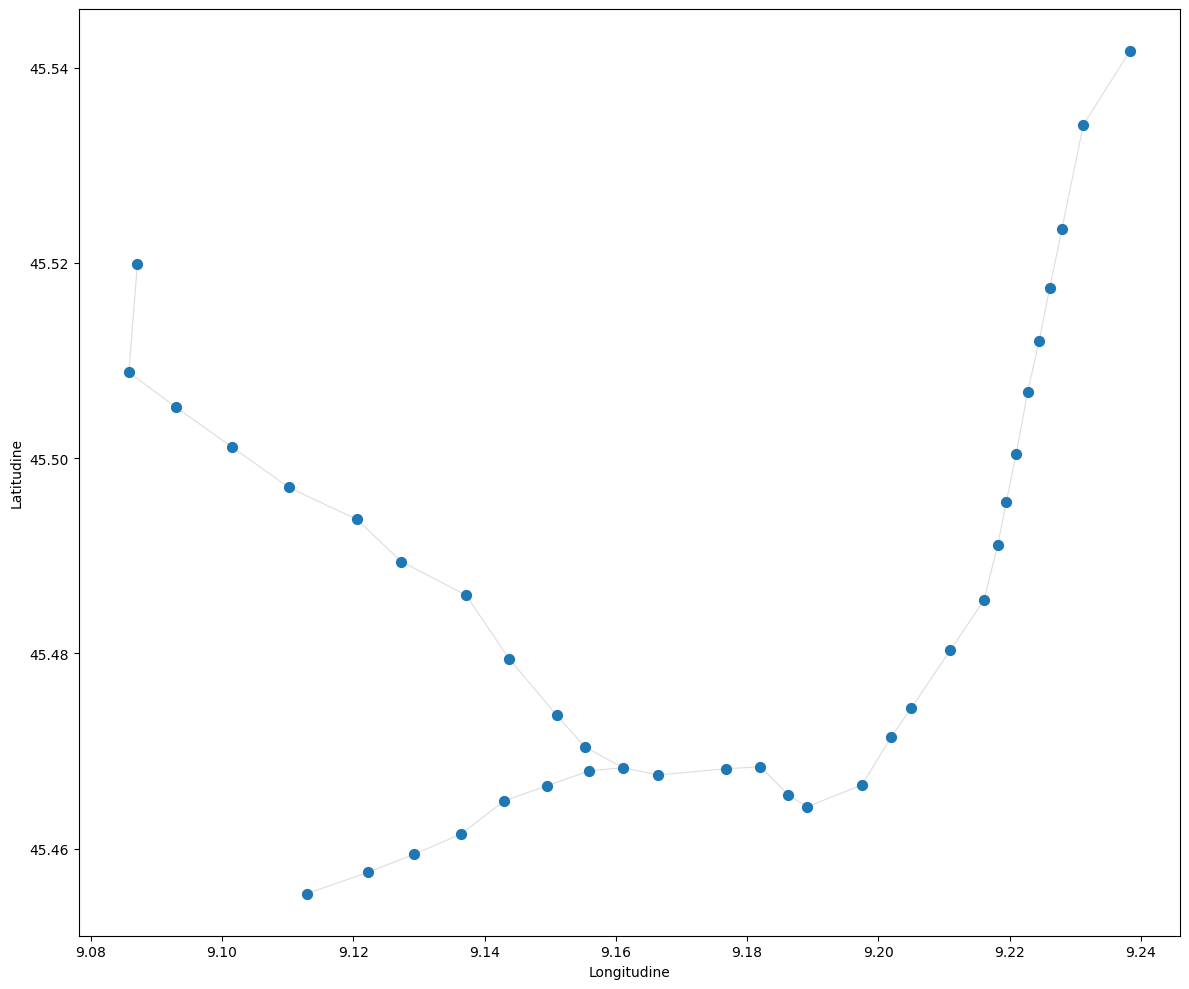
\includegraphics[width=\textwidth]{Immagini/Capitoli/cap3/rete_1.png}
    \caption{Linea 1}
    \label{fig:m1}
  \end{subfigure}%
  \hspace{0.03\textwidth}
  \begin{subfigure}[b]{0.40\textwidth}
    \centering
    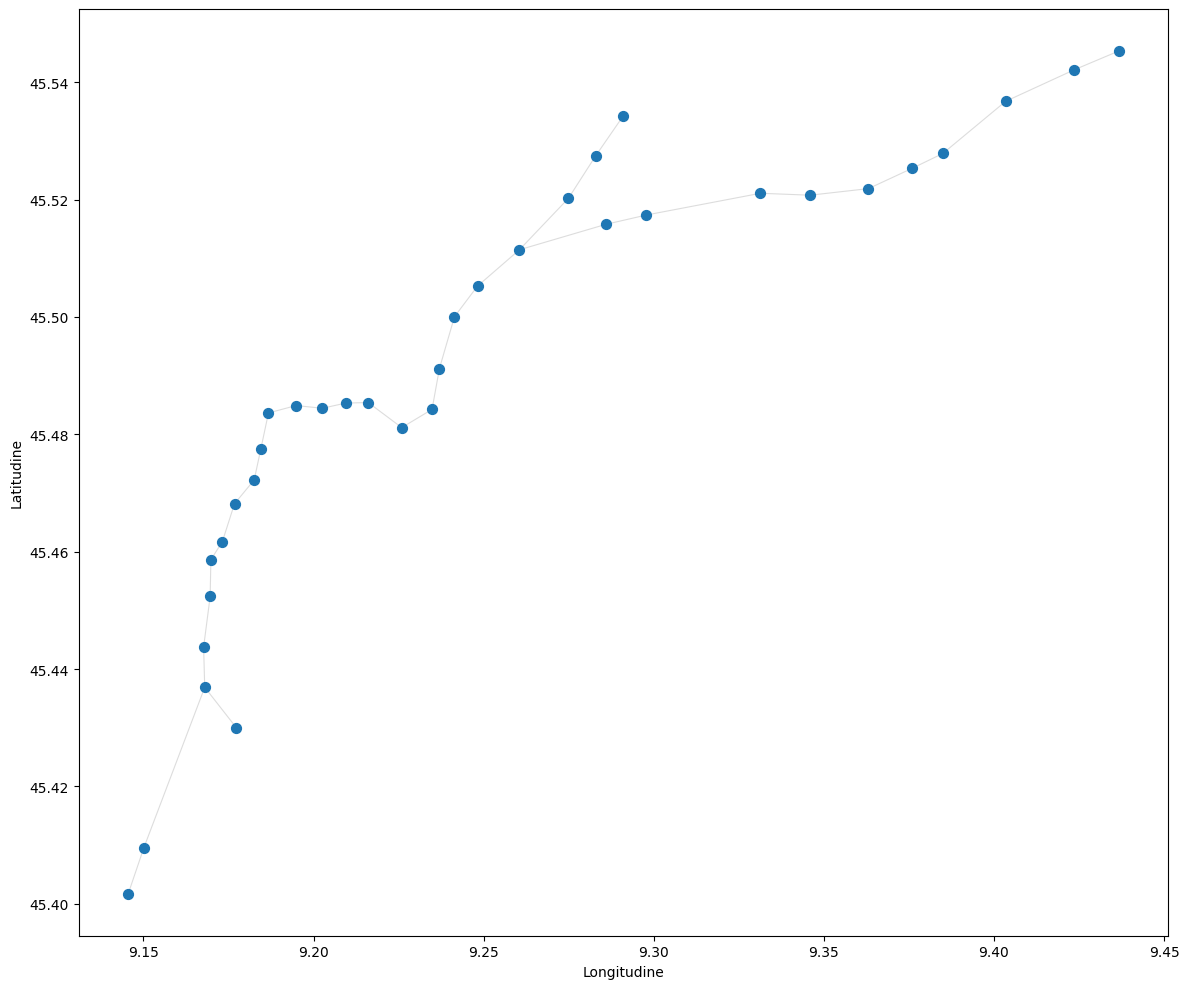
\includegraphics[width=\textwidth]{Immagini/Capitoli/cap3/rete_2.png}
    \caption{Linea 2}
    \label{fig:m2}
  \end{subfigure}

  % --- Riga 2 ---
  \vspace{0.02\textheight}
  \begin{subfigure}[b]{0.40\textwidth}
    \centering
    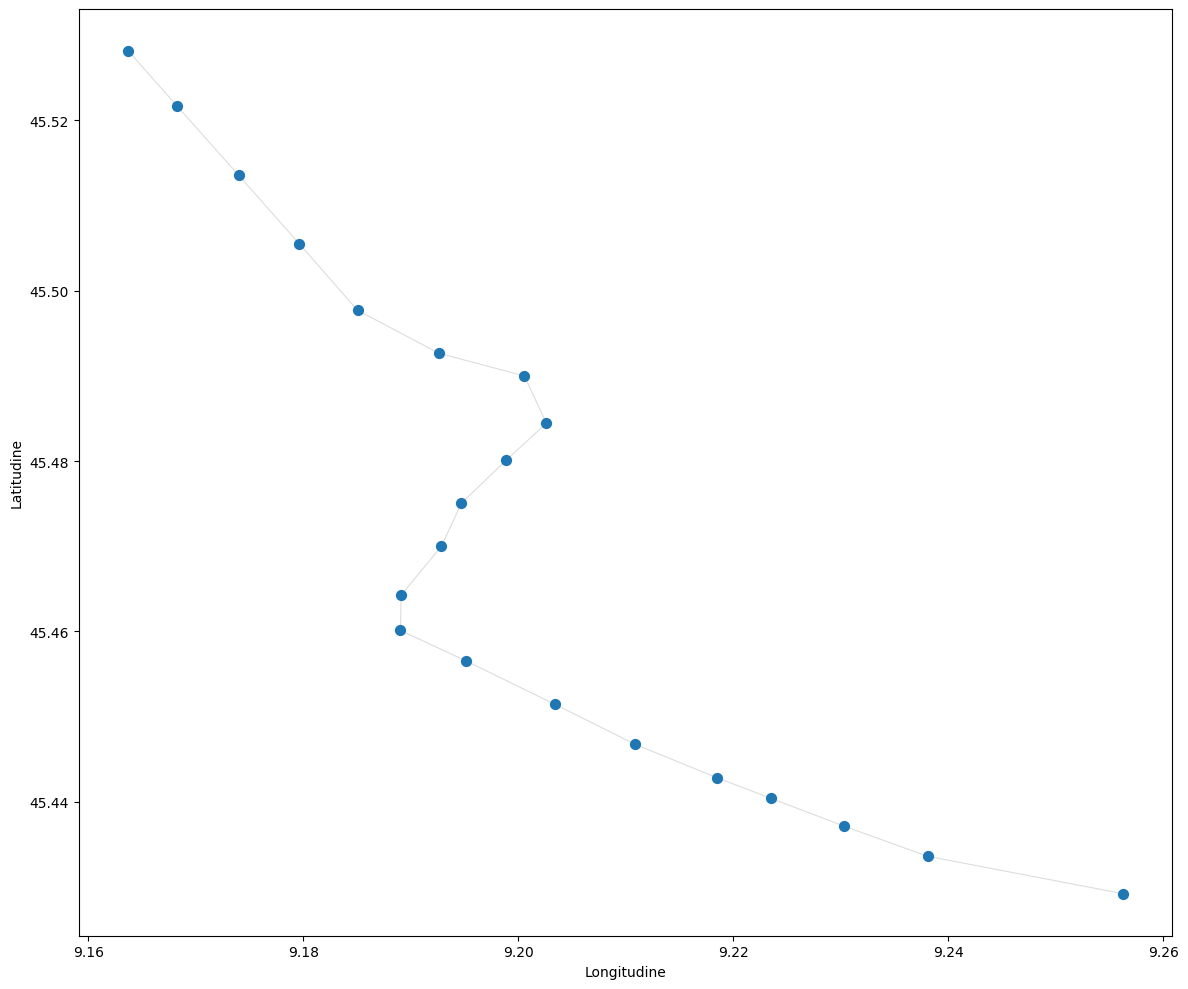
\includegraphics[width=\textwidth]{Immagini/Capitoli/cap3/rete_3.png}
    \caption{Linea 3}
    \label{fig:m3}
  \end{subfigure}%
  \hspace{0.03\textwidth}
  \begin{subfigure}[b]{0.40\textwidth}
    \centering
    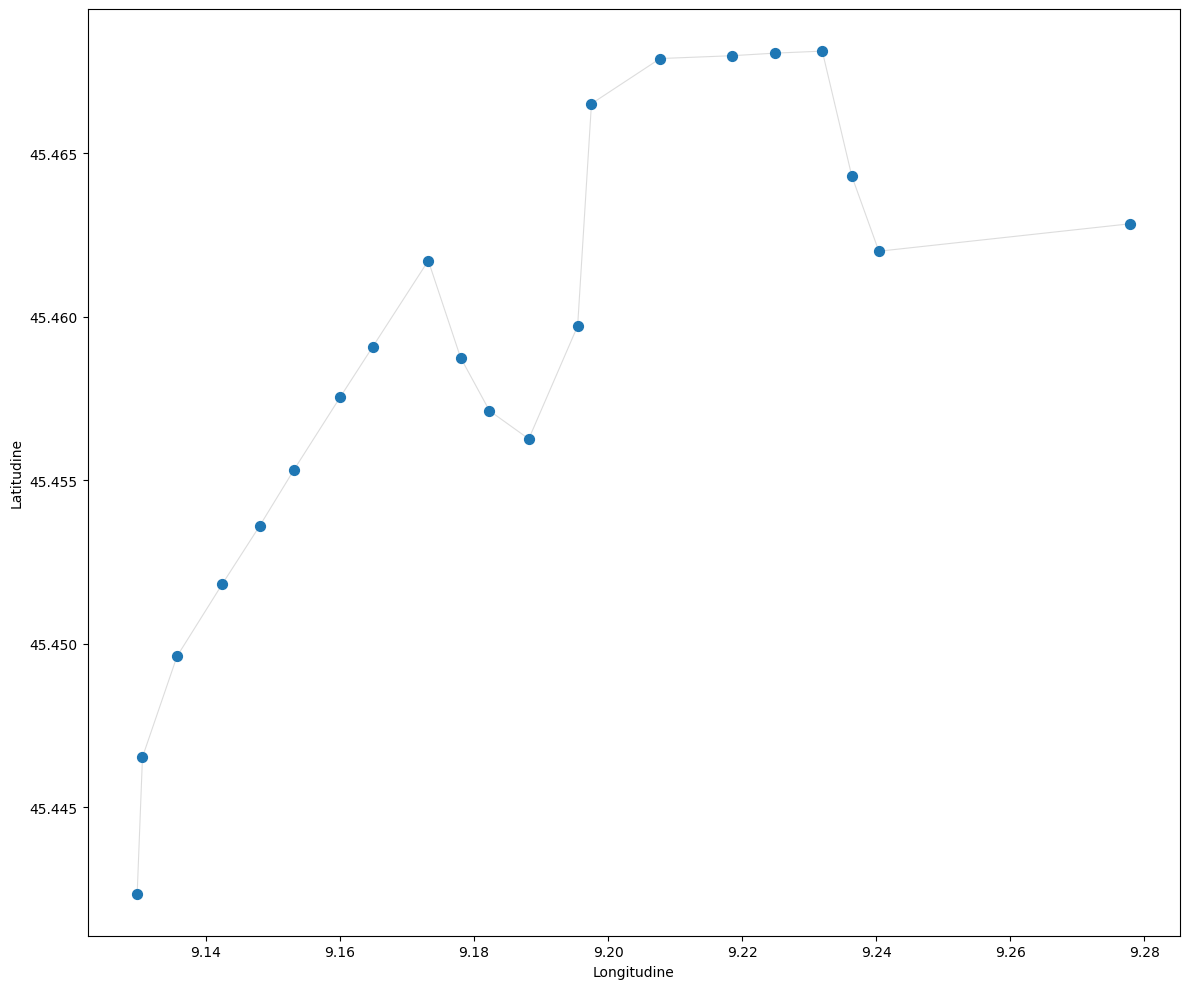
\includegraphics[width=\textwidth]{Immagini/Capitoli/cap3/rete_4.png}
    \caption{Linea 4}
    \label{fig:m4}
  \end{subfigure}

  % --- Riga 3 (centrata) ---
  \vspace{0.02\textheight}
  \begin{subfigure}[b]{0.40\textwidth}
    \centering
    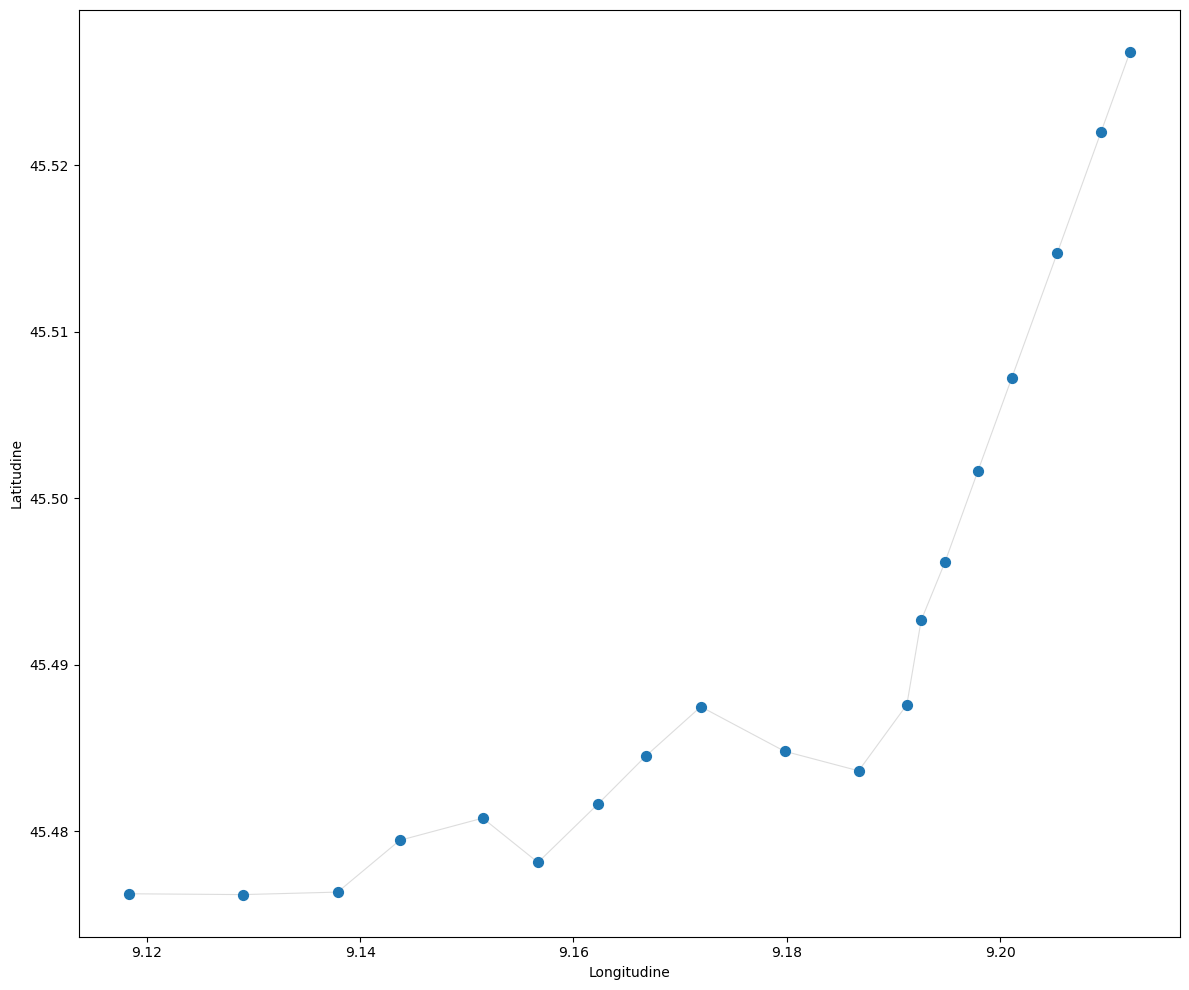
\includegraphics[width=\textwidth]{Immagini/Capitoli/cap3/rete_5.png}
    \caption{Linea 5}
    \label{fig:m5}
  \end{subfigure}

  % --- Didascalia generale ---
  \caption{Sottografi corrispondenti alle linee metropolitane.}
  \label{fig:sottografi}
\end{figure}

\section{Analisi dei nodi e degli archi}
Il grafo si compone di \textbf{125} nodi e \textbf{129} archi. Nella realtà, le stazioni sono 134 se contate singolarmente, ma si ricorda che nel grafo in studio le stazioni con nomenclature diverse ma fisicamente uguali sono state unite in un unico nodo. 

\vspace{1em}
\begin{table}[h!]
\centering
\begin{tabular}{l c c}
\hline
\textbf{Linea} & \textbf{Numero di vertici} & \textbf{Numero di archi} \\
\hline
Linea 1 & 38 & 37\\
Linea 2 & 35 & 34\\
Linea 3 & 21 & 20\\
Linea 4 & 21 & 20\\
Linea 5 & 19 & 18\\
\hline
\end{tabular}
\caption{Numero di vertici e archi per linea}
\label{tab: Numero di vertici e archi per linea}
\end{table}
\vspace{1em}

Nella tabella \ref{tab: Numero di vertici e archi per linea} sono presenti il numero di vertici e archi per ogni linea, in questo caso il numero di vertici corrisponde esattamente al numero di stazioni reali.

\section{Analisi dei gradi}
La rete presenta nodi con gradi che vanno da un minimo di \textbf{1}, ovvero i nodi capolinea, ad un massimo di \textbf{4} per i nodi di interscambio.

\vspace{1em}
\begin{table}[h!]
\centering
\begin{tabular}{l c c}
\hline
\textbf{Grado} & \textbf{Numero di vertici} & \textbf{Distribuzione} \\
\hline
1 & 13 & 10.4\% \\
2 & 100 & 80.0\% \\
3 & 3 & 2.4\% \\
4 & 9 & 7.2\% \\
\hline
\end{tabular}
\caption{Gradi dei nodi della rete}
\label{tab: Gradi dei nodi della rete}
\end{table}
\vspace{1em}

In tabella \ref{tab: Gradi dei nodi della rete} si può già notare che il grado più comune è il \textbf{2}, caratteristica tipica di \textbf{reti prevalentemente lineari} come quelle \textbf{metropolitane}, in cui ci sono diverse linee che si sviluppano radialmente con alcuni \textbf{interscambi} tipicamente situate al centro della rete. Questa caratteristica è fortemente visibile in figura \ref{fig: Distribuzione dei gradi dei nodi}.

\vspace{1em}
\begin{figure}[h!]
    \centering
    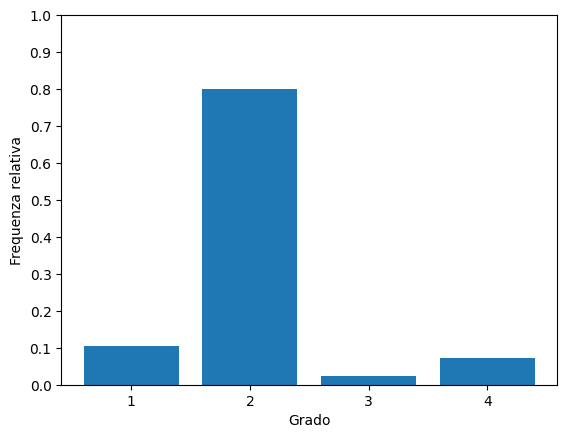
\includegraphics[width=0.5\linewidth]{Immagini//Capitoli//cap3/dist_gradi.png}
    \caption{Distribuzione dei gradi dei nodi}
    \label{fig: Distribuzione dei gradi dei nodi}
\end{figure}
\vspace{1em}

Gli unici nodi con grado \textbf{3} sono quelli di \textbf{diramazione}, caratteristiche delle linee \textit{1} e \textit{2} che si sviluppano in diversi rami, come evidenziato nelle figure \ref{fig:m1} e \ref{fig:m2}.

Da un punto di vista più formale, si ottengono le seguenti metriche:
\[
\begin{array}{cccc}
\hline
k_{\min} & k_{\max} & \langle k \rangle & \sigma_k \\
\hline
1 & 4 & 2.064 & 0.642 \\
\hline
\end{array}
\]

Il grado minimo indica la presenza di nodi terminali \textit{capolinea}, il grado massimo indica invece la presenza di nodi con al più 4 connessioni dirette. La rete non ha quindi degli \textit{hub} con una forte influenza, ma fungono comunque da nodi hub di interscambio.

Il grado medio è molto vicino a 2 e la deviazione standard è piuttosto bassa, confermando la presenza di molti nodi di grado 2.

\subsection{Distribuzione topografica dei gradi}
In figura \ref{fig: Distribuzione topologica dei gradi dei nodi} è rappresentata la distribuzione dei gradi da un punto di vista topografico, con i nodi colorati in base al proprio grado.

\vspace{1em}
\begin{figure}[h!]
    \centering
    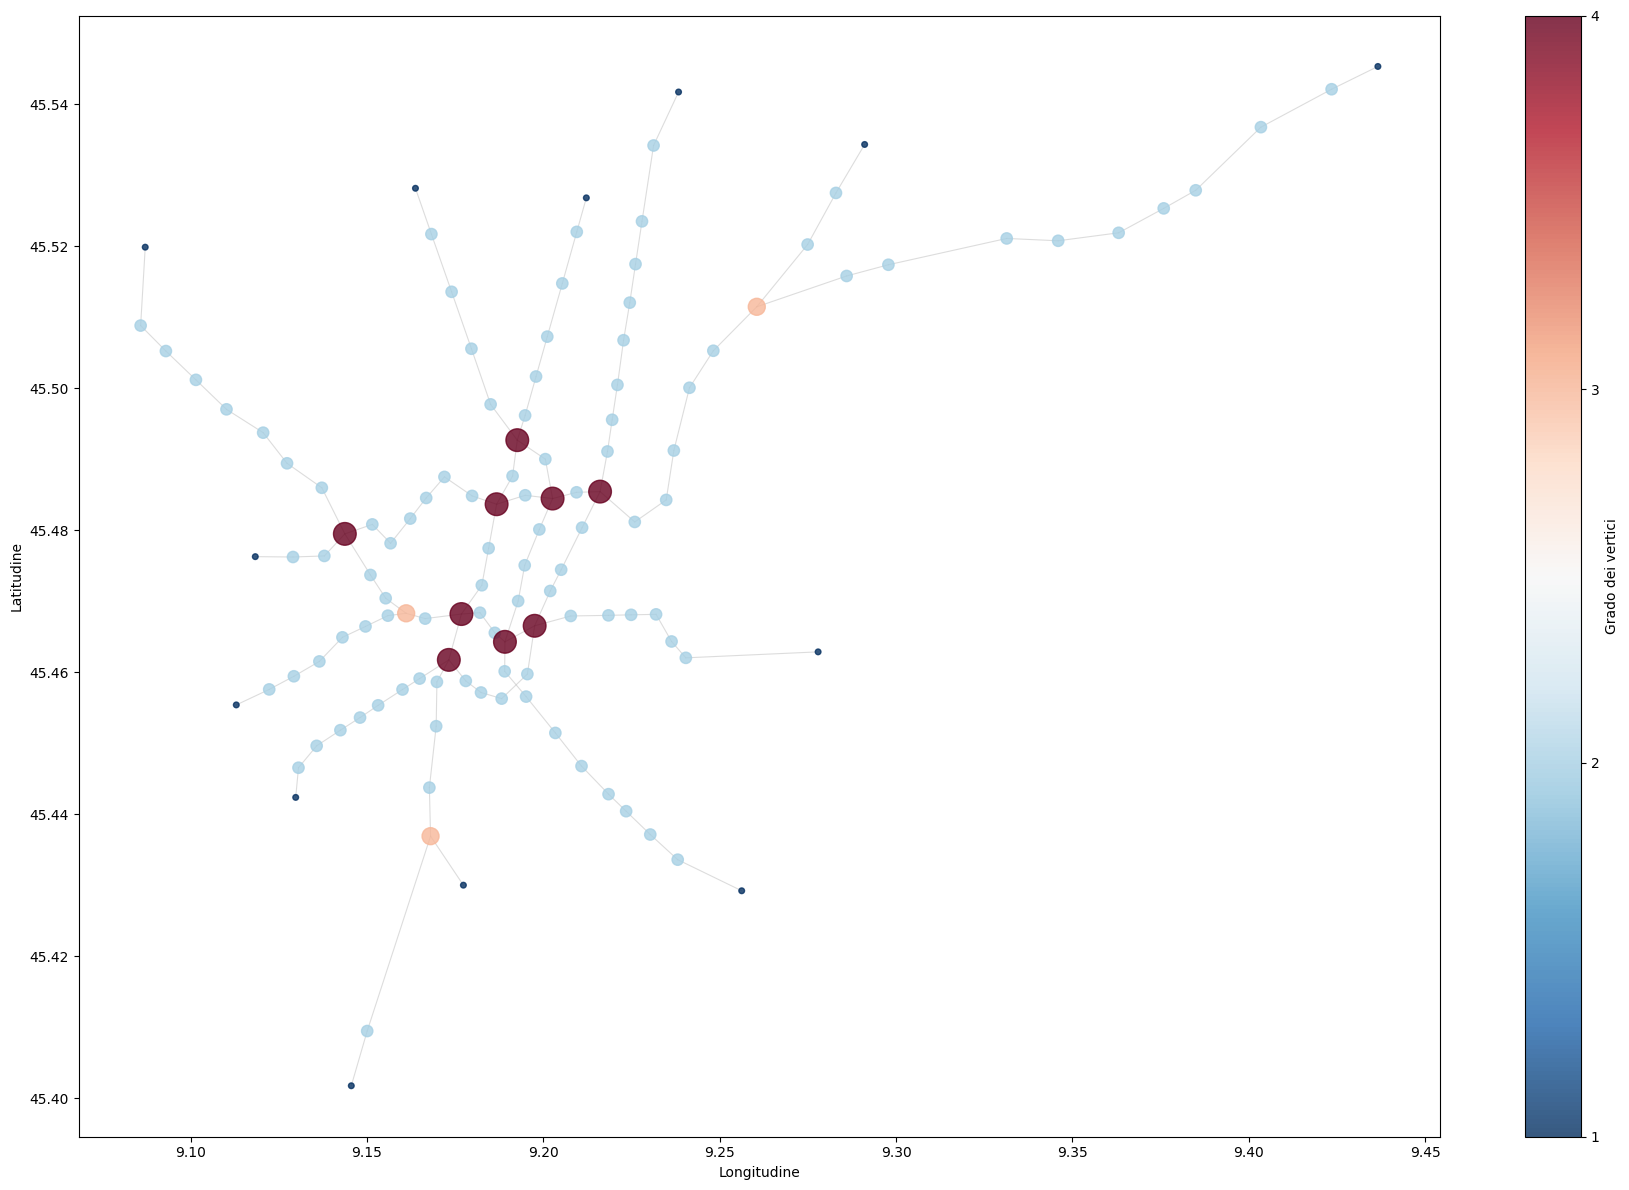
\includegraphics[width=0.8\linewidth]{Immagini//Capitoli//cap3/dist_gradi_mappa.png}
    \caption{Distribuzione topologica dei gradi dei nodi}
    \label{fig: Distribuzione topologica dei gradi dei nodi}
\end{figure}
\vspace{1em}

La rete mostra una configurazione \textit{radiale}, con diversi rami che si diramano dal centro verso la periferia, una struttura tipica delle reti metropolitane. \\
I nodi ad alto grado rappresentano snodi principali, dove convergono più linee, evidenti sono nella figura \ref{fig: Distribuzione topologica dei gradi dei nodi} le stazioni di \textit{Duomo} e \textit{Centrale FS}. I nodi periferici si trovano invece ai margini, coerentemente con il ruolo di \textit{capolinea}.

\section{Analisi dei cammini}
Le metriche principali calcolabili sui cammini sono riassunte di seguito.

\[
\begin{array}{cccc}
\hline
\mathrm{diam}(G) & \ell & E(G) & r(G) \\
\hline
35 & 12.101 & 0.1262 & 18 \\
\hline
\end{array}
\]

\subsection{Distanza massima e minima}
La \textbf{distanza massima} tra due nodi, ovvero il diametro $\mathrm{diam}(G)$ indica che le due stazioni più lontane nella rete sono separate da 35 fermate, il che rappresenta anche l'estensione complessiva della rete.

La \textbf{distanza minima}, ovvero la distanza dal nodo più centrale a quello più lontano chiamato raggio $r(G)$, indica che dal nodo più centrale si può raggiungere qualsiasi altra fermata con un cammino lungo al massimo 18.

\subsection{Distanza media minima}
In figura \ref{fig: Distribuzione dei cammini} sono rappresentate tutte le distanze minime tra coppie di nodi, ovvero di stazioni, della rete. La maggior parte dei nodi ha un cammino compreso tra 10 e 13, la coda destra mostra che esistono comunque coppie di nodi maggiormente distanti.


\vspace{1em}
\begin{figure}[h!]
    \centering
    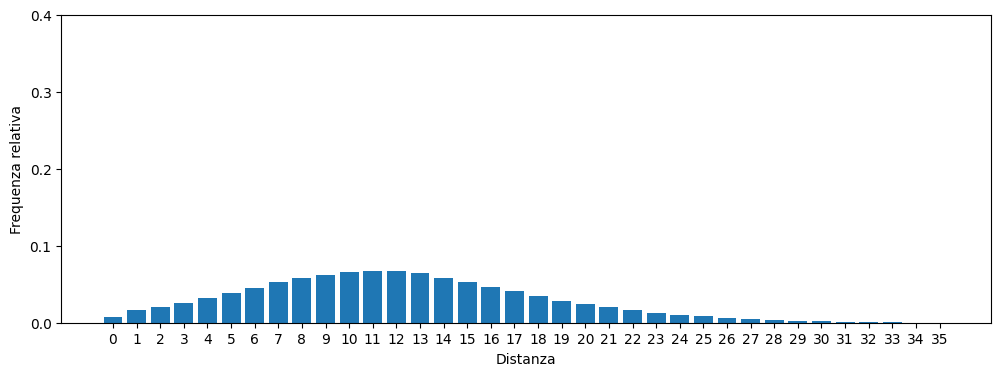
\includegraphics[width=0.8\linewidth]{Immagini//Capitoli//cap3/dist_cammini.png}
    \caption{Distribuzione dei cammini}
    \label{fig: Distribuzione dei cammini}
\end{figure}
\vspace{1em}

Quanto evidenziato in figura \ref{fig: Distribuzione dei cammini} si ritrova anche nella \textbf{lunghezza media dei cammini} $\ell$ di valore 12.101, coerente con il picco tra 10 e 13 del grafo.

\subsection{Efficienza globale}
L'efficienza globale $E(G)$ misura quanto efficacemente le informazioni, nel caso in studio i \textit{passeggeri}, possono muoversi attraverso la rete. Il valore di $0.13 \approx 0.1\text{--}0.3$ è tipico di infrastrutture \textbf{geografiche}, in cui i collegamenti devono seguire vincoli fisici e urbanistici.

\section{Analisi strutturale}

\subsection{Componenti connesse}
Essendo una PTN in cui ogni linea si intersceca con \textit{almeno un'altra} linea, la \textbf{componente connessa} è \textit{una}, ciò implica che la \textbf{giant component} corrisponde a tutta la rete.

\subsection{Clustering}
Una PTN metropolitana difficilmente presenta stazioni che godono della proprietà di \textit{transitività}, in linea con questa intuizione teorica nella PTN in studio il coefficiente di \textbf{clustering} è pari a \textit{zero}.

\subsection{Assortatività}
Con un \textbf{grado di Assortatività} di -0.0264, la rete è \textbf{disassortativa}, ovvero le stazioni molto connesse tendono a collegarsi a stazioni meno connesse, un comportamento tipico delle reti di trasporto in cui sono presenti \textit{hub} di \textit{modesta entità}, riportati in tabella \ref{tab: Hub score delle stazioni principali}, in uno struttura gerarchica fino ai nodi periferici.

\vspace{1em}
\begin{table}[h!]
\centering
\begin{tabular}{l c}
\hline
\textbf{Stazione} & \textbf{Hub Score} \\
\hline
Centrale FS & 1.000\\
Garibaldi FS & 0.967\\
Cadorna & 0.957\\
Zara & 0.850\\
Duomo & 0.829\\
\hline
\end{tabular}
\caption{Hub score delle stazioni principali}
\label{tab: Hub score delle stazioni principali}
\end{table}
\vspace{1em}

Quindi la rete è efficientemente organizzata per distribuzione del traffico, ma non molto robusta rispetto a guasti negli hub principali, aspetto che sarà \textbf{determinante} nello studio di vulnerabilità della rete nel capitolo \ref{cap5}.

